\section{Examples of scenario categories}
\label{sec:examples}

In this section, three different ways are presented to use the tags, presented in \cref{sec:tags}, for defining scenario categories. To illustrate this, we present three scenario categories\footnote{For more examples, we refer the reader to \autocite{degelder2019scenariocategories}.}. 

The first way to define a scenario category using tags is to list the tags that are applicable. To avoid ambiguity, first the top-level tag is mentioned and, next, the lower-level tags that apply. To illustrate this, see the scenario category ``driving on a straight road'' that is schematically shown in \cref{fig:scheme straight}.

\setlength{\figurewidth}{15em}
\begin{figure}[t]
	\centering
	% This file was created by tikzplotlib v0.8.7.
\begin{tikzpicture}

\definecolor{color0}{rgb}{0.8,1,0.8}
\definecolor{color1}{rgb}{0,0.4375,0.75}

\begin{axis}[
axis background/.style={fill=color0},
height=0.50\figurewidth,
scale only axis,
tick align=outside,
tick pos=left,
ticks=none,
width=\figurewidth,
x grid style={white!69.01960784313725!black},
xmin=-10, xmax=10,
xtick style={color=black},
y grid style={white!69.01960784313725!black},
ymin=-5, ymax=5,
ytick style={color=black}
]
\path [draw=white!80.0!black, fill=white!80.0!black]
(axis cs:-10,2.8)
--(axis cs:10,2.8)
--(axis cs:10,-2.8)
--(axis cs:-10,-2.8)
--cycle;
\addplot [semithick, black]
table {%
-10 2.8
10 2.8
};
\addplot [semithick, black]
table {%
10 -2.8
-10 -2.8
};
\addplot [semithick, black]
table {%
-10 0
-9.52380952380952 0
};
\addplot [semithick, black]
table {%
-7.61904761904762 0
-6.66666666666667 0
};
\addplot [semithick, black]
table {%
-4.76190476190476 0
-3.80952380952381 0
};
\addplot [semithick, black]
table {%
-1.90476190476191 0
-0.952380952380953 0
};
\addplot [semithick, black]
table {%
0.952380952380953 0
1.90476190476191 0
};
\addplot [semithick, black]
table {%
3.80952380952381 0
4.76190476190476 0
};
\addplot [semithick, black]
table {%
6.66666666666667 0
7.61904761904762 0
};
\addplot [semithick, black]
table {%
9.52380952380953 0
10 0
};
\path [draw=black, fill=color1]
(axis cs:-7.25,-1.39598214285714)
--(axis cs:-7.24189189189189,-0.873660714285714)
--(axis cs:-7.18513513513513,-0.672767857142857)
--(axis cs:-7.10405405405405,-0.600446428571429)
--(axis cs:-6.97432432432432,-0.552232142857143)
--(axis cs:-6.51216216216216,-0.495982142857143)
--(axis cs:-3.09864864864865,-0.536160714285714)
--(axis cs:-3.00945945945946,-0.592410714285714)
--(axis cs:-2.87162162162162,-0.769196428571428)
--(axis cs:-2.81486486486487,-0.962053571428571)
--(axis cs:-2.75,-1.39598214285714)
--(axis cs:-2.75,-1.40401785714286)
--(axis cs:-2.81486486486487,-1.83794642857143)
--(axis cs:-2.87162162162162,-2.03080357142857)
--(axis cs:-3.00945945945946,-2.20758928571429)
--(axis cs:-3.09864864864865,-2.26383928571429)
--(axis cs:-6.51216216216216,-2.30401785714286)
--(axis cs:-6.97432432432432,-2.24776785714286)
--(axis cs:-7.10405405405405,-2.19955357142857)
--(axis cs:-7.18513513513513,-2.12723214285714)
--(axis cs:-7.24189189189189,-1.92633928571429)
--(axis cs:-7.25,-1.40401785714286)
--cycle;
\path [draw=black, fill=color1]
(axis cs:-4.33108108108108,-0.568303571428571)
--(axis cs:-4.33918918918919,-0.367410714285714)
--(axis cs:-4.33108108108108,-0.319196428571428)
--(axis cs:-4.29864864864865,-0.343303571428571)
--(axis cs:-4.25,-0.552232142857143)
--cycle;
\path [draw=black, fill=color1]
(axis cs:-4.33108108108108,-2.23169642857143)
--(axis cs:-4.33918918918919,-2.43258928571429)
--(axis cs:-4.33108108108108,-2.48080357142857)
--(axis cs:-4.29864864864865,-2.45669642857143)
--(axis cs:-4.25,-2.24776785714286)
--cycle;
\path [draw=black, fill=white]
(axis cs:-6.71486486486486,-1.39598214285714)
--(axis cs:-6.69864864864865,-1.02633928571429)
--(axis cs:-6.65,-0.801339285714286)
--(axis cs:-6.58513513513514,-0.680803571428571)
--(axis cs:-6.52837837837838,-0.672767857142857)
--(axis cs:-6.01756756756757,-0.809375)
--(axis cs:-6.06621621621622,-0.945982142857143)
--(axis cs:-6.07432432432432,-1.15491071428571)
--(axis cs:-6.07432432432432,-1.64508928571429)
--(axis cs:-6.06621621621622,-1.85401785714286)
--(axis cs:-6.01756756756757,-1.990625)
--(axis cs:-6.52837837837838,-2.12723214285714)
--(axis cs:-6.58513513513514,-2.11919642857143)
--(axis cs:-6.65,-1.99866071428571)
--(axis cs:-6.69864864864865,-1.77366071428571)
--(axis cs:-6.71486486486486,-1.40401785714286)
--cycle;
\path [draw=black, fill=white]
(axis cs:-3.91756756756757,-1.39598214285714)
--(axis cs:-3.94189189189189,-0.962053571428571)
--(axis cs:-4.03108108108108,-0.688839285714286)
--(axis cs:-4.08783783783784,-0.632589285714286)
--(axis cs:-4.61486486486486,-0.841517857142857)
--(axis cs:-4.56621621621622,-1.034375)
--(axis cs:-4.55,-1.203125)
--(axis cs:-4.55,-1.596875)
--(axis cs:-4.56621621621622,-1.765625)
--(axis cs:-4.61486486486486,-1.95848214285714)
--(axis cs:-4.08783783783784,-2.16741071428571)
--(axis cs:-4.03108108108108,-2.11116071428571)
--(axis cs:-3.94189189189189,-1.83794642857143)
--(axis cs:-3.91756756756757,-1.40401785714286)
--cycle;
\path [draw=black, fill=white]
(axis cs:-6.02567567567568,-0.568303571428571)
--(axis cs:-5.81486486486487,-0.568303571428571)
--(axis cs:-5.81486486486487,-0.720982142857143)
--(axis cs:-5.92027027027027,-0.672767857142857)
--cycle;
\path [draw=black, fill=white]
(axis cs:-6.02567567567568,-2.23169642857143)
--(axis cs:-5.81486486486487,-2.23169642857143)
--(axis cs:-5.81486486486487,-2.07901785714286)
--(axis cs:-5.92027027027027,-2.12723214285714)
--cycle;
\path [draw=black, fill=white]
(axis cs:-5.76621621621622,-0.737053571428571)
--(axis cs:-5.76621621621622,-0.608482142857143)
--(axis cs:-5.73378378378378,-0.576339285714286)
--(axis cs:-5.20675675675676,-0.576339285714286)
--(axis cs:-5.18243243243243,-0.616517857142857)
--(axis cs:-5.23108108108108,-0.761160714285714)
--(axis cs:-5.30405405405405,-0.793303571428571)
--(axis cs:-5.57162162162162,-0.777232142857143)
--cycle;
\path [draw=black, fill=white]
(axis cs:-5.76621621621622,-2.06294642857143)
--(axis cs:-5.76621621621622,-2.19151785714286)
--(axis cs:-5.73378378378378,-2.22366071428571)
--(axis cs:-5.20675675675676,-2.22366071428571)
--(axis cs:-5.18243243243243,-2.18348214285714)
--(axis cs:-5.23108108108108,-2.03883928571429)
--(axis cs:-5.30405405405405,-2.00669642857143)
--(axis cs:-5.57162162162162,-2.02276785714286)
--cycle;
\path [draw=black, fill=white]
(axis cs:-5.15,-0.817410714285714)
--(axis cs:-5.02027027027027,-0.568303571428571)
--(axis cs:-4.28243243243243,-0.568303571428571)
--(axis cs:-4.29054054054054,-0.616517857142857)
--(axis cs:-4.70405405405405,-0.793303571428571)
--cycle;
\path [draw=black, fill=white]
(axis cs:-5.15,-1.98258928571429)
--(axis cs:-5.02027027027027,-2.23169642857143)
--(axis cs:-4.28243243243243,-2.23169642857143)
--(axis cs:-4.29054054054054,-2.18348214285714)
--(axis cs:-4.70405405405405,-2.00669642857143)
--cycle;
\path [draw=black, fill=white]
(axis cs:-3.2527027027027,-0.552232142857143)
--(axis cs:-3.09054054054054,-0.560267857142857)
--(axis cs:-2.96891891891892,-0.680803571428571)
--(axis cs:-2.91216216216216,-0.777232142857143)
--(axis cs:-2.89594594594595,-0.873660714285714)
--(axis cs:-2.89594594594595,-1.04241071428571)
--(axis cs:-2.98513513513514,-0.889732142857143)
--cycle;
\path [draw=black, fill=white]
(axis cs:-3.2527027027027,-2.24776785714286)
--(axis cs:-3.09054054054054,-2.23973214285714)
--(axis cs:-2.96891891891892,-2.11919642857143)
--(axis cs:-2.91216216216216,-2.02276785714286)
--(axis cs:-2.89594594594595,-1.92633928571429)
--(axis cs:-2.89594594594595,-1.75758928571429)
--(axis cs:-2.98513513513514,-1.91026785714286)
--cycle;
\addplot [black]
table {%
-6.63378378378378 -0.656696428571429
-6.86081081081081 -0.664732142857143
-7.07162162162162 -0.720982142857143
-7.13648648648649 -0.801339285714286
-7.13648648648649 -1.99866071428571
-7.07162162162162 -2.07901785714286
-6.86081081081081 -2.13526785714286
-6.63378378378378 -2.14330357142857
};
\addplot [black]
table {%
-3.00945945945946 -0.970089285714286
-2.98513513513514 -0.945982142857143
-2.89594594594595 -1.08258928571429
-2.89594594594595 -1.71741071428571
-2.98513513513514 -1.85401785714286
-3.00945945945946 -1.82991071428571
};
\addplot [black]
table {%
-3.26081081081081 -0.664732142857143
-4.0472972972973 -0.632589285714286
-3.00945945945946 -0.970089285714286
-3.00945945945946 -1.82991071428571
-4.0472972972973 -2.16741071428571
-3.26081081081081 -2.13526785714286
};
\addplot [semithick, red]
table {%
-2.75 -1.4
4.25 -1.4
};
\addplot [semithick, red]
table {%
3.5 -0.649999999999999
4.25 -1.4
3.5 -2.15
};
\end{axis}

\end{tikzpicture}

	\caption{Schematic overview for the scenario category ``driving on a straight road''.}
	\label{fig:scheme straight}
\end{figure}
\begin{figure}[t]
	\centering
	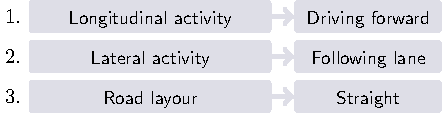
\includegraphics{figures/straight}
	\caption{Tags for the scenario category ``driving on a straight road''.}
	\label{fig:tags straight}
\end{figure}

It might be that the way to list the tags as shown in \cref{fig:tags straight} is too limited. For example, if multiple vehicles are involved, it might be useful to describe the activities of these vehicles separately. To accommodate this, a selection of tags of a scenario category may be grouped in order to indicate that these tags apply to the same actor. This is illustrated with the example shown in \cref{fig:scheme oncoming turning}: the scenario category ``oncoming vehicle turns right signalized junction''.
The ego vehicle is approaching a junction that is equipped with traffic light signals. The ego vehicle intends to go straight at the crossing. Another vehicle is approaching the junction from the opposite direction. The other vehicle intends to turn right at the junction, such that the trajectories of the other vehicle and the ego vehicle intersect. Note that right-hand traffic is assumed.
In \cref{fig:tags oncoming turning}, the corresponding tags are shown. The first part refers to the ego vehicle that intends to drive straight in forward direction. The second part refers to the other vehicle that turns right. The third part refers describes that the scenario happens at a signalized junction.


\setlength{\figurewidth}{15.0em}
\begin{figure}[t]
	\centering
	\input{figures/"oncoming vehicle right signalized.tikz"}
	\caption{Schematic overview for the scenario category ``oncoming vehicle turns right at signalized junction''. The blue vehicle denotes the ego vehicle.}
	\label{fig:scheme oncoming turning}
\end{figure}
\begin{figure}[t]
	\centering
	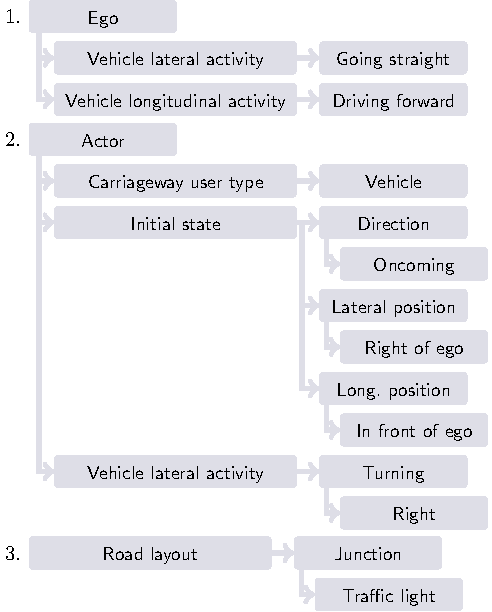
\includegraphics{figures/oncoming_turning}
	\caption{Tags for the scenario category ``oncoming vehicle turns right at signalized junction''.}
	\label{fig:tags oncoming turning}
\end{figure}

A third way to define a scenario category using tags is presented in case the order in which the tags apply matter. To illustrate this, consider the scenario category ``cut in at merging lanes'' that is schematically shown in \cref{fig:scheme cut in}. 
Another vehicle is driving in the same direction as the ego vehicle in an adjacent lane. The other vehicle makes a lane change because the lanes are merging. In \cref{fig:tags cut in}, the corresponding tags are shown. Most notably, the tag for the ``lead vehicle'' changes from ``no leader'' to ``leader. Note that the direction of the lane change is not described. This could mean that the vehicle could either change lane to the left or to the right. In any case, this actor becomes the lead vehicle, as described my the tag ``lead vehicle''. 

\setlength{\figurewidth}{22.5em}
\begin{figure}[t]
	\centering
	% This file was created by matplotlib2tikz v0.7.5.
\begin{tikzpicture}

\definecolor{color0}{rgb}{0.8,1,0.8}
\definecolor{color1}{rgb}{0,0.4375,0.75}

\begin{axis}[
axis background/.style={fill=color0},
height=0.33\figurewidth,
scale only axis,
tick align=outside,
tick pos=left,
ticks=none,
width=\figurewidth,
x grid style={white!69.01960784313725!black},
xmin=-15, xmax=15,
xtick style={color=black},
y grid style={white!69.01960784313725!black},
ymin=-5, ymax=5,
ytick style={color=black}
]
\path [draw=white!80.0!black, fill=white!80.0!black]
(axis cs:-14.9995238848361,2.79999995952042)
--(axis cs:0.0860615228589551,2.79743478949463)
--(axis cs:5.14664116816982,1.39487383099742)
--(axis cs:4.95111961061006,-2.79829127699914)
--(axis cs:0.0851092925312272,-2.80256512954621)
--(axis cs:-15.0004761151639,-2.79999995952042)
--cycle;
\path [draw=white, fill=white]
(axis cs:-13.7375163208298,1.54978534825388)
--(axis cs:-13.7375673331688,1.24978535259098)
--(axis cs:-12.107552053032,1.33950818424803)
--(axis cs:-12.052562256295,1.27949883285331)
--(axis cs:-12.0150775605388,1.18949245761206)
--(axis cs:-12.0150877630066,1.12949245847948)
--(axis cs:-12.3550877580912,1.12955027246366)
--(axis cs:-11.882643878495,0.79946993280057)
--(axis cs:-11.2375877742469,1.12936025150094)
--(axis cs:-11.7875877662956,1.12945377412242)
--(axis cs:-11.78756736136,1.24945377238758)
--(axis cs:-11.8250520571161,1.33946014762882)
--(axis cs:-11.9200316508071,1.45947629980133)
--cycle;
\path [draw=white, fill=white]
(axis cs:-8.71307612613488,1.54893098675345)
--(axis cs:-8.71312713847387,1.24893099109055)
--(axis cs:-7.08311185833707,1.3386538227476)
--(axis cs:-7.0281220616,1.27864447135287)
--(axis cs:-6.99063736584383,1.18863809611163)
--(axis cs:-6.99064756831163,1.12863809697905)
--(axis cs:-7.33064756339625,1.12869591096323)
--(axis cs:-6.85820368380007,0.798615571300139)
--(axis cs:-6.21314757955194,1.12850589000051)
--(axis cs:-6.7631475716006,1.12859941262199)
--(axis cs:-6.763127166665,1.24859941088715)
--(axis cs:-6.80061186242117,1.33860578612839)
--(axis cs:-6.89559145611216,1.4586219383009)
--cycle;
\path [draw=white, fill=white]
(axis cs:-3.68863593143991,1.54807662525302)
--(axis cs:-3.6886869437789,1.24807662959012)
--(axis cs:-2.0586716636421,1.33779946124717)
--(axis cs:-2.00368186690503,1.27779010985244)
--(axis cs:-1.96619717114886,1.1877837346112)
--(axis cs:-1.96620737361666,1.12778373547862)
--(axis cs:-2.30620736870128,1.1278415494628)
--(axis cs:-1.8337634891051,0.797761209799709)
--(axis cs:-1.18870738485697,1.12765152850008)
--(axis cs:-1.73870737690563,1.12774505112156)
--(axis cs:-1.73868697197003,1.24774504938672)
--(axis cs:-1.7761716677262,1.33775142462796)
--(axis cs:-1.87115126141719,1.45776757680047)
--cycle;
\path [draw=white, fill=white]
(axis cs:1.33580426325506,1.54722226375259)
--(axis cs:1.33575325091607,1.24722226808969)
--(axis cs:2.96576853105287,1.33694509974674)
--(axis cs:3.02075832778994,1.27693574835201)
--(axis cs:3.05824302354611,1.18692937311077)
--(axis cs:3.05823282107831,1.12692937397819)
--(axis cs:2.71823282599369,1.12698718796237)
--(axis cs:3.19067670558987,0.796906848299277)
--(axis cs:3.835732809838,1.12679716699965)
--(axis cs:3.28573281778934,1.12689068962112)
--(axis cs:3.28575322272494,1.24689068788629)
--(axis cs:3.24826852696877,1.33689706312753)
--(axis cs:3.15328893327778,1.45691321530004)
--cycle;
\path [draw=white!80.0!black, fill=white!80.0!black]
(axis cs:5.14664116816982,1.39487383099742)
--(axis cs:10,0)
--(axis cs:15,0)
--(axis cs:15,-2.8)
--(axis cs:10,-2.8)
--(axis cs:4.95111961061006,-2.79829127699914)
--cycle;
\addplot [semithick, black]
table {%
-14.9995238848361 2.79999995952042
0.0860615228589551 2.79743478949463
5.14664116816982 1.39487383099742
};
\addplot [semithick, black]
table {%
4.95111961061006 -2.79829127699914
0.0851092925312272 -2.80256512954621
-15.0004761151639 -2.79999995952042
};
\addplot [semithick, black]
table {%
-15 0
-14.5214818862195 -8.13677619457745e-05
};
\addplot [semithick, black]
table {%
-12.6074094310976 -0.000406838809728873
-11.6503732035367 -0.000569574333620422
};
\addplot [semithick, black]
table {%
-9.73630074841479 -0.00089504538140352
-8.77926452085385 -0.00105778090529507
};
\addplot [semithick, black]
table {%
-6.86519206573195 -0.00138325195307817
-5.90815583817101 -0.00154598747696972
};
\addplot [semithick, black]
table {%
-3.99408338304911 -0.00187145852475281
-3.03704715548817 -0.00203419404864436
};
\addplot [semithick, black]
table {%
-1.12297470036627 -0.00235966509642746
-0.165938472805329 -0.00252240062031901
};
\addplot [semithick, black]
table {%
1.74813398231657 -0.00284787166810215
2.70517020987751 -0.00301060719199373
};
\addplot [semithick, black]
table {%
4.6192426649994 -0.00333607823977688
5.09776077877988 -0.00341744600172267
};
\addplot [semithick, white]
table {%
-13.7375163208298 1.54978534825388
-13.7375673331688 1.24978535259098
-12.107552053032 1.33950818424803
-12.052562256295 1.27949883285331
-12.0150775605388 1.18949245761206
-12.0150877630066 1.12949245847948
-12.3550877580912 1.12955027246366
-11.882643878495 0.79946993280057
-11.2375877742469 1.12936025150094
-11.7875877662956 1.12945377412242
-11.78756736136 1.24945377238758
-11.8250520571161 1.33946014762882
-11.9200316508071 1.45947629980133
-13.7375163208298 1.54978534825388
};
\addplot [semithick, white]
table {%
-8.71307612613488 1.54893098675345
-8.71312713847387 1.24893099109055
-7.08311185833707 1.3386538227476
-7.0281220616 1.27864447135287
-6.99063736584383 1.18863809611163
-6.99064756831163 1.12863809697905
-7.33064756339625 1.12869591096323
-6.85820368380007 0.798615571300139
-6.21314757955194 1.12850589000051
-6.7631475716006 1.12859941262199
-6.763127166665 1.24859941088715
-6.80061186242117 1.33860578612839
-6.89559145611216 1.4586219383009
-8.71307612613488 1.54893098675345
};
\addplot [semithick, white]
table {%
-3.68863593143991 1.54807662525302
-3.6886869437789 1.24807662959012
-2.0586716636421 1.33779946124717
-2.00368186690503 1.27779010985244
-1.96619717114886 1.1877837346112
-1.96620737361666 1.12778373547862
-2.30620736870128 1.1278415494628
-1.8337634891051 0.797761209799709
-1.18870738485697 1.12765152850008
-1.73870737690563 1.12774505112156
-1.73868697197003 1.24774504938672
-1.7761716677262 1.33775142462796
-1.87115126141719 1.45776757680047
-3.68863593143991 1.54807662525302
};
\addplot [semithick, white]
table {%
1.33580426325506 1.54722226375259
1.33575325091607 1.24722226808969
2.96576853105287 1.33694509974674
3.02075832778994 1.27693574835201
3.05824302354611 1.18692937311077
3.05823282107831 1.12692937397819
2.71823282599369 1.12698718796237
3.19067670558987 0.796906848299277
3.835732809838 1.12679716699965
3.28573281778934 1.12689068962112
3.28575322272494 1.24689068788629
3.24826852696877 1.33689706312753
3.15328893327778 1.45691321530004
1.33580426325506 1.54722226375259
};
\addplot [semithick, black]
table {%
5.14664116816982 1.39487383099742
10 0
15 0
};
\addplot [semithick, black]
table {%
15 -2.8
10 -2.8
4.95111961061006 -2.79829127699914
};
\path [draw=black, fill=color1]
(axis cs:-12.25,-1.39598214285714)
--(axis cs:-12.2418918918919,-0.873660714285714)
--(axis cs:-12.1851351351351,-0.672767857142857)
--(axis cs:-12.1040540540541,-0.600446428571429)
--(axis cs:-11.9743243243243,-0.552232142857143)
--(axis cs:-11.5121621621622,-0.495982142857143)
--(axis cs:-8.09864864864865,-0.536160714285714)
--(axis cs:-8.00945945945946,-0.592410714285714)
--(axis cs:-7.87162162162162,-0.769196428571428)
--(axis cs:-7.81486486486487,-0.962053571428571)
--(axis cs:-7.75,-1.39598214285714)
--(axis cs:-7.75,-1.40401785714286)
--(axis cs:-7.81486486486487,-1.83794642857143)
--(axis cs:-7.87162162162162,-2.03080357142857)
--(axis cs:-8.00945945945946,-2.20758928571429)
--(axis cs:-8.09864864864865,-2.26383928571429)
--(axis cs:-11.5121621621622,-2.30401785714286)
--(axis cs:-11.9743243243243,-2.24776785714286)
--(axis cs:-12.1040540540541,-2.19955357142857)
--(axis cs:-12.1851351351351,-2.12723214285714)
--(axis cs:-12.2418918918919,-1.92633928571429)
--(axis cs:-12.25,-1.40401785714286)
--cycle;
\path [draw=black, fill=color1]
(axis cs:-9.33108108108108,-0.568303571428571)
--(axis cs:-9.33918918918919,-0.367410714285714)
--(axis cs:-9.33108108108108,-0.319196428571428)
--(axis cs:-9.29864864864865,-0.343303571428571)
--(axis cs:-9.25,-0.552232142857143)
--cycle;
\path [draw=black, fill=color1]
(axis cs:-9.33108108108108,-2.23169642857143)
--(axis cs:-9.33918918918919,-2.43258928571429)
--(axis cs:-9.33108108108108,-2.48080357142857)
--(axis cs:-9.29864864864865,-2.45669642857143)
--(axis cs:-9.25,-2.24776785714286)
--cycle;
\path [draw=black, fill=white]
(axis cs:-11.7148648648649,-1.39598214285714)
--(axis cs:-11.6986486486486,-1.02633928571429)
--(axis cs:-11.65,-0.801339285714286)
--(axis cs:-11.5851351351351,-0.680803571428571)
--(axis cs:-11.5283783783784,-0.672767857142857)
--(axis cs:-11.0175675675676,-0.809375)
--(axis cs:-11.0662162162162,-0.945982142857143)
--(axis cs:-11.0743243243243,-1.15491071428571)
--(axis cs:-11.0743243243243,-1.64508928571429)
--(axis cs:-11.0662162162162,-1.85401785714286)
--(axis cs:-11.0175675675676,-1.990625)
--(axis cs:-11.5283783783784,-2.12723214285714)
--(axis cs:-11.5851351351351,-2.11919642857143)
--(axis cs:-11.65,-1.99866071428571)
--(axis cs:-11.6986486486486,-1.77366071428571)
--(axis cs:-11.7148648648649,-1.40401785714286)
--cycle;
\path [draw=black, fill=white]
(axis cs:-8.91756756756757,-1.39598214285714)
--(axis cs:-8.94189189189189,-0.962053571428571)
--(axis cs:-9.03108108108108,-0.688839285714286)
--(axis cs:-9.08783783783784,-0.632589285714286)
--(axis cs:-9.61486486486486,-0.841517857142857)
--(axis cs:-9.56621621621622,-1.034375)
--(axis cs:-9.55,-1.203125)
--(axis cs:-9.55,-1.596875)
--(axis cs:-9.56621621621622,-1.765625)
--(axis cs:-9.61486486486486,-1.95848214285714)
--(axis cs:-9.08783783783784,-2.16741071428571)
--(axis cs:-9.03108108108108,-2.11116071428571)
--(axis cs:-8.94189189189189,-1.83794642857143)
--(axis cs:-8.91756756756757,-1.40401785714286)
--cycle;
\path [draw=black, fill=white]
(axis cs:-11.0256756756757,-0.568303571428571)
--(axis cs:-10.8148648648649,-0.568303571428571)
--(axis cs:-10.8148648648649,-0.720982142857143)
--(axis cs:-10.9202702702703,-0.672767857142857)
--cycle;
\path [draw=black, fill=white]
(axis cs:-11.0256756756757,-2.23169642857143)
--(axis cs:-10.8148648648649,-2.23169642857143)
--(axis cs:-10.8148648648649,-2.07901785714286)
--(axis cs:-10.9202702702703,-2.12723214285714)
--cycle;
\path [draw=black, fill=white]
(axis cs:-10.7662162162162,-0.737053571428571)
--(axis cs:-10.7662162162162,-0.608482142857143)
--(axis cs:-10.7337837837838,-0.576339285714286)
--(axis cs:-10.2067567567568,-0.576339285714286)
--(axis cs:-10.1824324324324,-0.616517857142857)
--(axis cs:-10.2310810810811,-0.761160714285714)
--(axis cs:-10.3040540540541,-0.793303571428571)
--(axis cs:-10.5716216216216,-0.777232142857143)
--cycle;
\path [draw=black, fill=white]
(axis cs:-10.7662162162162,-2.06294642857143)
--(axis cs:-10.7662162162162,-2.19151785714286)
--(axis cs:-10.7337837837838,-2.22366071428571)
--(axis cs:-10.2067567567568,-2.22366071428571)
--(axis cs:-10.1824324324324,-2.18348214285714)
--(axis cs:-10.2310810810811,-2.03883928571429)
--(axis cs:-10.3040540540541,-2.00669642857143)
--(axis cs:-10.5716216216216,-2.02276785714286)
--cycle;
\path [draw=black, fill=white]
(axis cs:-10.15,-0.817410714285714)
--(axis cs:-10.0202702702703,-0.568303571428571)
--(axis cs:-9.28243243243243,-0.568303571428571)
--(axis cs:-9.29054054054054,-0.616517857142857)
--(axis cs:-9.70405405405405,-0.793303571428571)
--cycle;
\path [draw=black, fill=white]
(axis cs:-10.15,-1.98258928571429)
--(axis cs:-10.0202702702703,-2.23169642857143)
--(axis cs:-9.28243243243243,-2.23169642857143)
--(axis cs:-9.29054054054054,-2.18348214285714)
--(axis cs:-9.70405405405405,-2.00669642857143)
--cycle;
\path [draw=black, fill=white]
(axis cs:-8.2527027027027,-0.552232142857143)
--(axis cs:-8.09054054054054,-0.560267857142857)
--(axis cs:-7.96891891891892,-0.680803571428571)
--(axis cs:-7.91216216216216,-0.777232142857143)
--(axis cs:-7.89594594594595,-0.873660714285714)
--(axis cs:-7.89594594594595,-1.04241071428571)
--(axis cs:-7.98513513513513,-0.889732142857143)
--cycle;
\path [draw=black, fill=white]
(axis cs:-8.2527027027027,-2.24776785714286)
--(axis cs:-8.09054054054054,-2.23973214285714)
--(axis cs:-7.96891891891892,-2.11919642857143)
--(axis cs:-7.91216216216216,-2.02276785714286)
--(axis cs:-7.89594594594595,-1.92633928571429)
--(axis cs:-7.89594594594595,-1.75758928571429)
--(axis cs:-7.98513513513513,-1.91026785714286)
--cycle;
\path [draw=black, fill=red]
(axis cs:-7.25,1.40401785714286)
--(axis cs:-7.24189189189189,1.92633928571429)
--(axis cs:-7.18513513513513,2.12723214285714)
--(axis cs:-7.10405405405405,2.19955357142857)
--(axis cs:-6.97432432432432,2.24776785714286)
--(axis cs:-6.51216216216216,2.30401785714286)
--(axis cs:-3.09864864864865,2.26383928571429)
--(axis cs:-3.00945945945946,2.20758928571429)
--(axis cs:-2.87162162162162,2.03080357142857)
--(axis cs:-2.81486486486487,1.83794642857143)
--(axis cs:-2.75,1.40401785714286)
--(axis cs:-2.75,1.39598214285714)
--(axis cs:-2.81486486486487,0.962053571428571)
--(axis cs:-2.87162162162162,0.769196428571429)
--(axis cs:-3.00945945945946,0.592410714285714)
--(axis cs:-3.09864864864865,0.536160714285714)
--(axis cs:-6.51216216216216,0.495982142857143)
--(axis cs:-6.97432432432432,0.552232142857143)
--(axis cs:-7.10405405405405,0.600446428571428)
--(axis cs:-7.18513513513513,0.672767857142857)
--(axis cs:-7.24189189189189,0.873660714285714)
--(axis cs:-7.25,1.39598214285714)
--cycle;
\path [draw=black, fill=red]
(axis cs:-4.33108108108108,2.23169642857143)
--(axis cs:-4.33918918918919,2.43258928571429)
--(axis cs:-4.33108108108108,2.48080357142857)
--(axis cs:-4.29864864864865,2.45669642857143)
--(axis cs:-4.25,2.24776785714286)
--cycle;
\path [draw=black, fill=red]
(axis cs:-4.33108108108108,0.568303571428571)
--(axis cs:-4.33918918918919,0.367410714285714)
--(axis cs:-4.33108108108108,0.319196428571428)
--(axis cs:-4.29864864864865,0.343303571428571)
--(axis cs:-4.25,0.552232142857143)
--cycle;
\path [draw=black, fill=white]
(axis cs:-6.71486486486486,1.40401785714286)
--(axis cs:-6.69864864864865,1.77366071428571)
--(axis cs:-6.65,1.99866071428571)
--(axis cs:-6.58513513513514,2.11919642857143)
--(axis cs:-6.52837837837838,2.12723214285714)
--(axis cs:-6.01756756756757,1.990625)
--(axis cs:-6.06621621621622,1.85401785714286)
--(axis cs:-6.07432432432432,1.64508928571429)
--(axis cs:-6.07432432432432,1.15491071428571)
--(axis cs:-6.06621621621622,0.945982142857143)
--(axis cs:-6.01756756756757,0.809375)
--(axis cs:-6.52837837837838,0.672767857142857)
--(axis cs:-6.58513513513514,0.680803571428571)
--(axis cs:-6.65,0.801339285714285)
--(axis cs:-6.69864864864865,1.02633928571429)
--(axis cs:-6.71486486486486,1.39598214285714)
--cycle;
\path [draw=black, fill=white]
(axis cs:-3.91756756756757,1.40401785714286)
--(axis cs:-3.94189189189189,1.83794642857143)
--(axis cs:-4.03108108108108,2.11116071428571)
--(axis cs:-4.08783783783784,2.16741071428571)
--(axis cs:-4.61486486486486,1.95848214285714)
--(axis cs:-4.56621621621622,1.765625)
--(axis cs:-4.55,1.596875)
--(axis cs:-4.55,1.203125)
--(axis cs:-4.56621621621622,1.034375)
--(axis cs:-4.61486486486486,0.841517857142857)
--(axis cs:-4.08783783783784,0.632589285714286)
--(axis cs:-4.03108108108108,0.688839285714286)
--(axis cs:-3.94189189189189,0.962053571428571)
--(axis cs:-3.91756756756757,1.39598214285714)
--cycle;
\path [draw=black, fill=white]
(axis cs:-6.02567567567568,2.23169642857143)
--(axis cs:-5.81486486486487,2.23169642857143)
--(axis cs:-5.81486486486487,2.07901785714286)
--(axis cs:-5.92027027027027,2.12723214285714)
--cycle;
\path [draw=black, fill=white]
(axis cs:-6.02567567567568,0.568303571428571)
--(axis cs:-5.81486486486487,0.568303571428571)
--(axis cs:-5.81486486486487,0.720982142857143)
--(axis cs:-5.92027027027027,0.672767857142857)
--cycle;
\path [draw=black, fill=white]
(axis cs:-5.76621621621622,2.06294642857143)
--(axis cs:-5.76621621621622,2.19151785714286)
--(axis cs:-5.73378378378378,2.22366071428571)
--(axis cs:-5.20675675675676,2.22366071428571)
--(axis cs:-5.18243243243243,2.18348214285714)
--(axis cs:-5.23108108108108,2.03883928571429)
--(axis cs:-5.30405405405405,2.00669642857143)
--(axis cs:-5.57162162162162,2.02276785714286)
--cycle;
\path [draw=black, fill=white]
(axis cs:-5.76621621621622,0.737053571428571)
--(axis cs:-5.76621621621622,0.608482142857143)
--(axis cs:-5.73378378378378,0.576339285714286)
--(axis cs:-5.20675675675676,0.576339285714286)
--(axis cs:-5.18243243243243,0.616517857142857)
--(axis cs:-5.23108108108108,0.761160714285714)
--(axis cs:-5.30405405405405,0.793303571428571)
--(axis cs:-5.57162162162162,0.777232142857143)
--cycle;
\path [draw=black, fill=white]
(axis cs:-5.15,1.98258928571429)
--(axis cs:-5.02027027027027,2.23169642857143)
--(axis cs:-4.28243243243243,2.23169642857143)
--(axis cs:-4.29054054054054,2.18348214285714)
--(axis cs:-4.70405405405405,2.00669642857143)
--cycle;
\path [draw=black, fill=white]
(axis cs:-5.15,0.817410714285714)
--(axis cs:-5.02027027027027,0.568303571428571)
--(axis cs:-4.28243243243243,0.568303571428571)
--(axis cs:-4.29054054054054,0.616517857142857)
--(axis cs:-4.70405405405405,0.793303571428571)
--cycle;
\path [draw=black, fill=white]
(axis cs:-3.2527027027027,2.24776785714286)
--(axis cs:-3.09054054054054,2.23973214285714)
--(axis cs:-2.96891891891892,2.11919642857143)
--(axis cs:-2.91216216216216,2.02276785714286)
--(axis cs:-2.89594594594595,1.92633928571429)
--(axis cs:-2.89594594594595,1.75758928571429)
--(axis cs:-2.98513513513514,1.91026785714286)
--cycle;
\path [draw=black, fill=white]
(axis cs:-3.2527027027027,0.552232142857143)
--(axis cs:-3.09054054054054,0.560267857142857)
--(axis cs:-2.96891891891892,0.680803571428571)
--(axis cs:-2.91216216216216,0.777232142857143)
--(axis cs:-2.89594594594595,0.873660714285714)
--(axis cs:-2.89594594594595,1.04241071428571)
--(axis cs:-2.98513513513514,0.889732142857143)
--cycle;
\addplot [black]
table {%
-11.6337837837838 -0.656696428571429
-11.8608108108108 -0.664732142857143
-12.0716216216216 -0.720982142857143
-12.1364864864865 -0.801339285714286
-12.1364864864865 -1.99866071428571
-12.0716216216216 -2.07901785714286
-11.8608108108108 -2.13526785714286
-11.6337837837838 -2.14330357142857
};
\addplot [black]
table {%
-8.00945945945946 -0.970089285714286
-7.98513513513513 -0.945982142857143
-7.89594594594595 -1.08258928571429
-7.89594594594595 -1.71741071428571
-7.98513513513513 -1.85401785714286
-8.00945945945946 -1.82991071428571
};
\addplot [black]
table {%
-8.26081081081081 -0.664732142857143
-9.0472972972973 -0.632589285714286
-8.00945945945946 -0.970089285714286
-8.00945945945946 -1.82991071428571
-9.0472972972973 -2.16741071428571
-8.26081081081081 -2.13526785714286
};
\addplot [semithick, red]
table {%
-7.75 -1.4
-2.75 -1.4
};
\addplot [semithick, red]
table {%
-3.5 -0.649999999999999
-2.75 -1.4
-3.5 -2.15
};
\addplot [black]
table {%
-6.63378378378378 2.14330357142857
-6.86081081081081 2.13526785714286
-7.07162162162162 2.07901785714286
-7.13648648648649 1.99866071428571
-7.13648648648649 0.801339285714285
-7.07162162162162 0.720982142857143
-6.86081081081081 0.664732142857143
-6.63378378378378 0.656696428571428
};
\addplot [black]
table {%
-3.00945945945946 1.82991071428571
-2.98513513513514 1.85401785714286
-2.89594594594595 1.71741071428571
-2.89594594594595 1.08258928571429
-2.98513513513514 0.945982142857143
-3.00945945945946 0.970089285714286
};
\addplot [black]
table {%
-3.26081081081081 2.13526785714286
-4.0472972972973 2.16741071428571
-3.00945945945946 1.82991071428571
-3.00945945945946 0.970089285714286
-4.0472972972973 0.632589285714286
-3.26081081081081 0.664732142857143
};
\addplot [semithick, red]
table {%
-2.75 1.4
-0.75 1.4
-0.434210526315789 1.38090582476381
-0.118421052631579 1.32414413838089
0.197368421052632 1.23126325168908
0.513157894736842 1.10479671315495
0.828947368421053 0.948194200276037
1.14473684210526 0.765727421371397
1.46052631578947 0.562373594514157
1.77631578947368 0.343679681997119
2.09210526315789 0.115611083661265
2.40789473684211 -0.115611083661265
2.72368421052632 -0.343679681997119
3.03947368421053 -0.562373594514157
3.35526315789474 -0.765727421371398
3.67105263157895 -0.948194200276037
3.98684210526316 -1.10479671315495
4.30263157894737 -1.23126325168908
4.61842105263158 -1.32414413838089
4.93421052631579 -1.38090582476381
5.25 -1.4
7.25 -1.4
};
\addplot [semithick, red]
table {%
6.5 -0.65
7.25 -1.4
6.5 -2.15
};
\end{axis}

\end{tikzpicture}
	\caption{Schematic overview for the scenario category ``cut in at merging lanes''. The blue vehicle denotes the ego vehicle.}
	\label{fig:scheme cut in}		
\end{figure}
\begin{figure}[t]
	\centering
	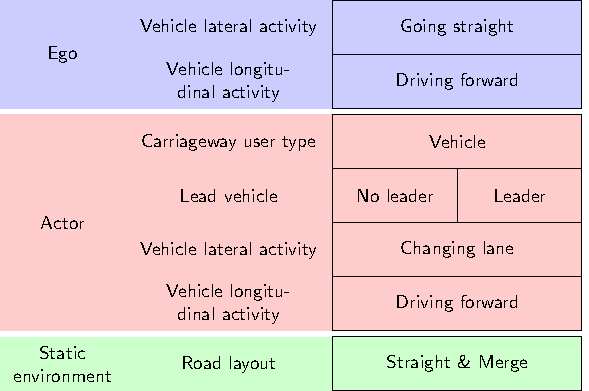
\includegraphics[width=\linewidth]{figures/cut-in_tags}
	\caption{Tags for the scenario category ``cut in at merging lanes''.}
	\label{fig:tags cut in}
\end{figure}



